\section{Spot The Bot}

In this section, we first provide an overview of the \emph{Spot The Bot} framework and then describe the individual steps of the evaluation process.

\subsection{Overview}
% figure
%----------------------------------------------------------------------------
\begin{figure*}
    \centering
    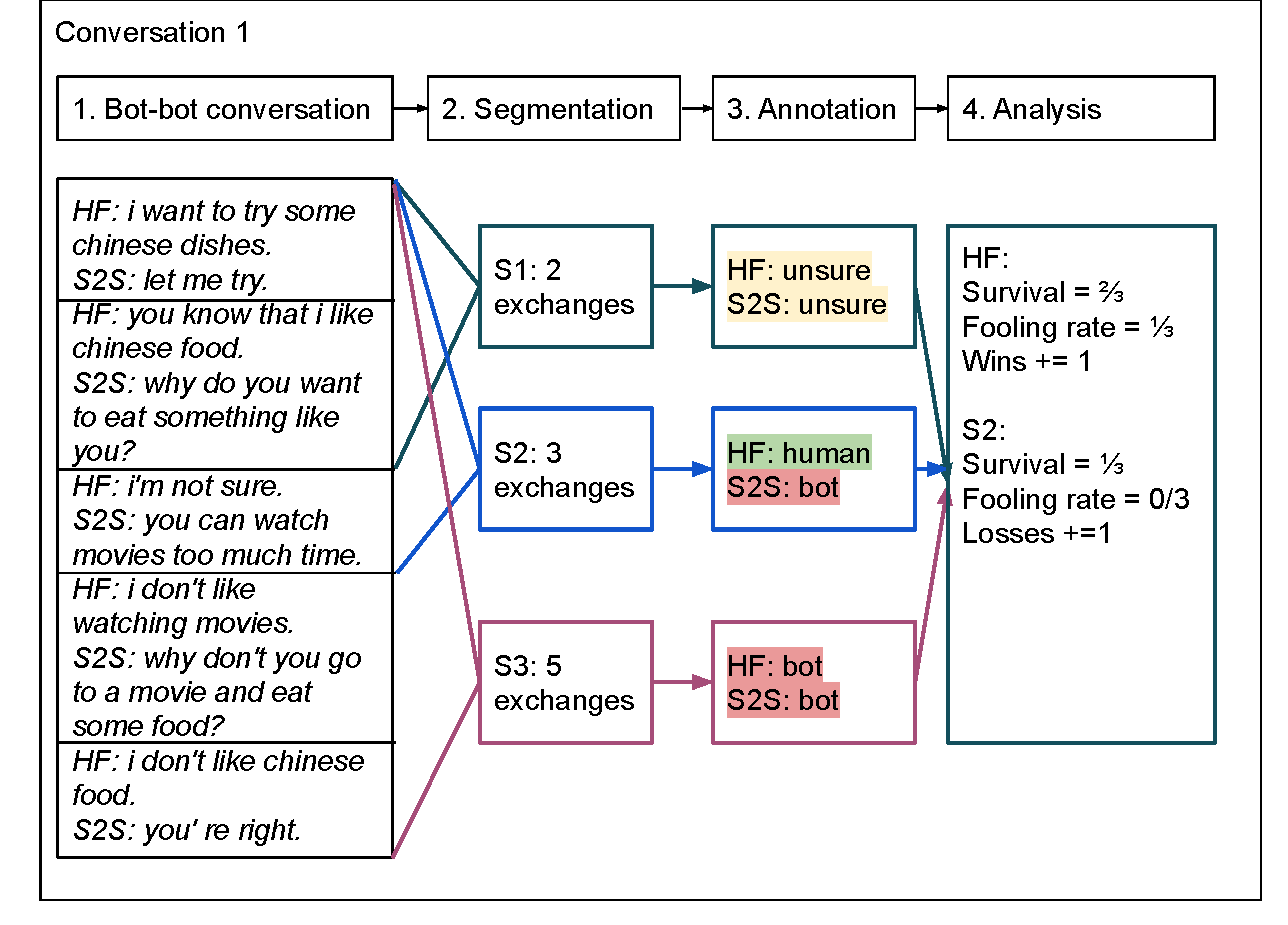
\includegraphics[width=0.7\linewidth]{figures/Spot the bot - annotation example - sketch3.pdf}
    \caption{Overview of the Spot The Bot process. 1: A bot-bot conversation is segmented into sub-segments of different lengths (2, 3, and 5 exchanges). 2: These are show to distinct sets of annotators who judge whether each entity is a bot. 4: The winner is determined for each annotated segment. This process is repeated for all conversations between the competing bots. 5: Finally, wins are aggregated from all annotated segments for each bot to create a ranking. *TODO make this figure prettier; find better visual presentation.}
    \label{fig:example}
\end{figure*}
%----------------------------------------------------------------------------
\emph{Spot The Bot} employs a tournament among conversational dialogue systems (bots) to determine which performs the best at mimicking the conversational behaviour of humans. To measure the success of each bot, human crowdworkers are shown conversations between the competing bots, mixed with conversations between humans. The crowdworkers' task is then to determine for each participant in a conversation whether it is a human or a bot (or whether they are unsure). The bot that is most frequently annotated as being human, wins the tournament. Figure \ref{fig:example} provides an overview of the process for one conversation.

More formally, assume that there is a pool of $B$ bots $\{B_1, ..., B_B\}$, which is to be ranked, e.g.\ when a novel dialogue strategy is to be compared against existing strategies. For each pair of bots, a set of conversations is sampled by letting the bots talk to each other, where $S_{ij}$ denotes the set of conversations between $B_i$ and $B_j$. Each conversation is defined as a sequence of exchanges $e_0, ..., e_N$, where each exchange consists of two turns, one per entity $e_i = \{t_0^{e_i}, t_1^{e_i}\}$.

%\emph{Spot The Bot} employs an annotation task that lets human crowdworkers read a conversation and decide for each entity in the conversation if it is a human or a bot. 
%The bot-bot conversations are then shown to human crowdworkers who determine for each participant in a conversation whether it is a bot or a human.
Showing only bot-bot conversations to the crowdworkers raises two issues: First, many conversational dialogue systems are not yet human-like enough to fool humans. Second, the crowdworkers might soon realize that all conversations are among bots, thus, classifying all entities as bots. 
To alleviate the first issue, we add a time component under the assumption that disguising as humans in shorter conversations is achievable also for weaker bots. Hence, we segment the conversations into different stages: $e_0, ..., e_i$, as shown in Figure \ref{fig:example}. The bots are then differentiated not only by their ability to fool humans, but also by how long they are able to pass as a human (or at least are not spotted as a bot). For the second issue, we add conversations between humans into the pool. These serve two purposes: first, as distractors, so that the crowdworkers cannot classify all entities as bots, and second, as an upper bound for evaluating the human-like behaviour of the competing bots.
Additionally, the framework allows to rate specific features, which are often used in current human evaluation (e.g. fluency, appropriateness, ...). The framework then measures the influence of these features on the survival time of the bots. 
%Additionally, we ask the crowdworkers to state which bot performed better with regards to certain features: fluency, sensibleness, and specificity as defined in \cite{adiwardana2020towards}. 
To rank the bots, we apply two different analysis on the annotation outcome: pair-wise ranking (rank the bots based on pair-wise comparisons from the annotated conversations), and survival analysis (i.e. probability of survival at each exchange and the influence of the different features).

\subsection{Rating Process}\label{sec:setting}

\paragraph{Bot-Bot Conversations.} For each pair of bots $B_i$, $B_j$ in the pool, we sample $|S_{ij}|$ conversations. In order to prime the conversations and obtain some variety of dialogues in $S_{ij}$.Given a set of contexts in the test set, the conversations are primed by showing the context to the bots. However, the initial context is not shown to the crowdworkers during annotation, since they are written by humans and are not part of the bot output. %The length of the sampled conversation is based on the conversation lengths in the given domain. This is to avoid that the bots are spotted by simply looking at the conversation length. 
%\paragraph{Human-Bot Conversations.} Ideally, our approach works without relying on human-bot conversations, which are costly to obtain and often very noisy if not executed with care. We show that our approach works without the need of human-bot conversations, by comparing the results of the \emph{Spot The Bot} annotation procedure with and without human-bot conversations. For this, we collected human-bot conversations for each bot by letting members of our lab converse with them. We instructed them to adhere to the dialogue style of the respective domain and to avoid being adversarial. 
\paragraph{Segmentation.} In order to simulate the time component, we show the conversations at different stages $e_0, ..., e_i$, where we chose different sets of values for $i$ depending on the domain\footnote{We experimented with letting crowdworkers decide themselves when to decide the exchange at which they were sure that an entity in the conversation is a bot or a human. However, this approach required too much fine-tuning to elicit the desired behaviour, cf.\ Appendix \ref{sec:appendix_gamification}.}. Each segment of the same conversation is annotated by different annotators to avoid that one annotator sees different segments of the same conversation. We assign two workers per conversation segment to be able to analyze their agreement.
\paragraph{Annotation.} The generated bot-bot conversations and a set of randomly sampled human-human conversations are presented to crowdworkers. The crowdworkers are presented with a conversation segment and have to decide for each entity if it is a human or a bot. There is an option for "unsure" as well, since we want to avoid forcing random decisions when annotators are not confident.%are interested in cases where annotators are sure about their decision. 
\paragraph{Features.} There are two decisions to be made for the features: which features to rate (fluency, adequacy, quality, sensibleness, ... ) and how to rate them (Likert scale, continuous scale, pairwise comparison, ...).
